\section{Prototypes}

Our primary focus within social insurance is on pension insurance, we have ported the most important components of the german pension system to ethereum in our surveys and from our experience and theories we have also developed a decentralised pension system that is independent of country and company.

\subsection{German Pension System}

In order to demonstrate the potential of blockchain-based social security, we created a prototype based on the model of the german statutory pay-as-you-go pension system. To demonstrate that blockchain can solve problems globally, we also developed a prototype of a global pension system which is fully decentralized and neither in the hands of governments nor any insurance companies.

The Asure dApp will become the reference implementation for dApps using the Asure protocol and platform. 
\newline\newline
It will feature
\begin{itemize}
\item a technical feasibility study of the german statutory pension system implemented on the Ethereum blockchain and the Asure protocol / platform.
\item a complete wallet implementation.
\item an overview and management of your insurance policies.
\item an insurance store to find and buy insurance policies.
\end{itemize}

Please try out the Asure dApp which runs currently on the Ethereum Rinkiby testnet: 
https://dapp.asure.io

\subsection{Decentralized Pension System}

This is an alpha experiment to show how social security systems can be improved in the future with the help of blockchain technology.
\newline\newline
The idea is to implement a pay-as-you-go pension system. Members pay their contributions in ETH and receive ERC20 tokens in return. No contributions are invested on the capital market and therefore no interest is earned. Instead, the paid-in ETH are used directly for the payment of outstanding pension claims. How much pension is paid out depends on how many pension token a pensioner has, e.g. how many contributions he paid into the system.
\newline\newline
As a rule, pay-as-you-go systems only work because, for example, states introduce mandatory social security systems and can thus guarantee a stable number of members and contribution payments. In a decentralised pension system nobody can be forced to become a member. Instead, we want to incentivize membership by

\begin{itemize}
\item Giving people who join early, more bonus
\item Paying people a higher pension if they made higher contributions
\item Paying people a longer pension if they contributed for a long time
\end{itemize}

\begin{figure}[H]
    \centering
    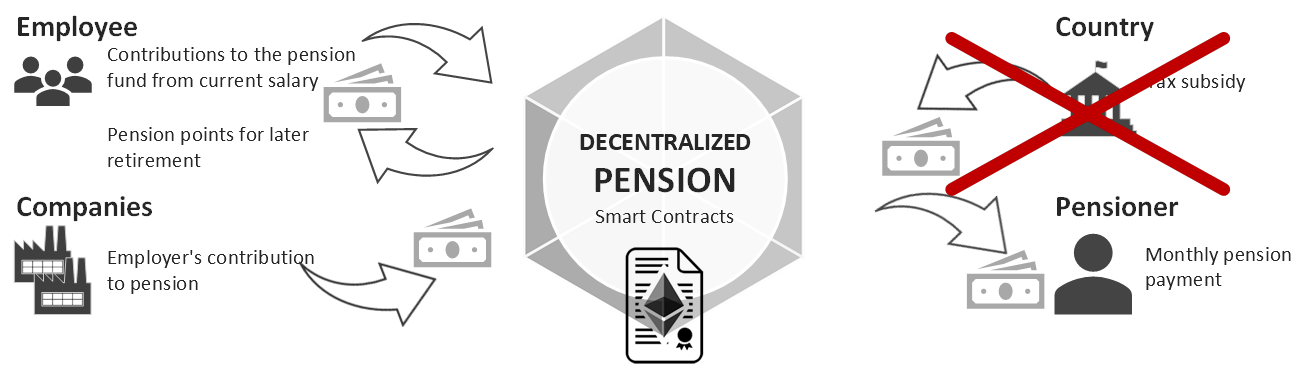
\includegraphics[width=5.0in]{pension.png}
    \caption{PAYG Model}
    \label{fig:payg}
\end{figure}

Please try out the Asure decentralized pension which runs currently on the Ethereum Rinkiby testnet: 
https://ethberlin.asure.io 
\newline\newline

\textbf{How much bonus i get as an early adopter?}

\begin{eqnarray}
	DTP_{bonus} = f(year) = 1.5-0.12 * log(year)
\end{eqnarray}

\begin{figure}[H]
    \centering
    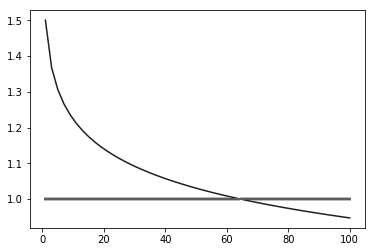
\includegraphics[width=3.0in]{pension_bonus.png}
    \caption{Decentralized pension bonus by year}
    \label{fig:pension_bonus}
\end{figure}

\textbf{How long pension can be recieved?}

The idea of using a quadratic function is, to incentivize people to pay 40 years if possible.

\begin{eqnarray}
	targetMonths =  12 \cdot 40 years
\end{eqnarray}

\begin{eqnarray}
	entitlementMonths = \frac{payedMonths^2}{targetMonths}
\end{eqnarray}

\begin{figure}[H]
    \centering
    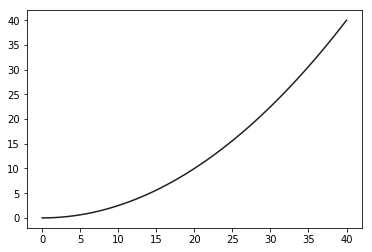
\includegraphics[width=3.0in]{pension_years.png}
    \caption{Decentralized pension payed vs. recive years}
    \label{fig:pension_years}
\end{figure}

\textbf{How much decentralized pension token can i get?}

\begin{eqnarray}
	DPT = \begin{cases} 1 + \frac{amount-amount_{max}}
	{targetPrice - amount_{max}} 
	* DTP_{bonus} & amount \geq targetPrice\\
	\frac{amount - amount_{min}}
	{targetPrice - amount_{min}} 
	* DTP_{bonus} & otherwise\end{cases}
\end{eqnarray}

\begin{eqnarray}
targetPrice - amount_{max} \neq 0 \quad and \quad targetPrice - amount_{min} \neq 0
\end{eqnarray}

\textbf{How payout will work?}

The goal is to reward the last in case everyone leaves the system.
\newline\newline

\textbf{Benefits}

\begin{itemize}
\item no organisation fee 
\item global
\item transparent
\item independent
\item open-source
\end{itemize}
